%%%%%%%%%%%%%%%%%%%%%%%%%%%%%%%%%%%%%%%%%%%%%%%%%%%%%%%%%%%%%%%%%
%
% Project     : Turnverein App
% Title       : 
% File        : umsetzung.tex Rev. 00
% Date        : 07.07.14
% Author      : Raffael Santschi
%
%%%%%%%%%%%%%%%%%%%%%%%%%%%%%%%%%%%%%%%%%%%%%%%%%%%%%%%%%%%%%%%%%

\chapter{Umsetzung des Prototypen}\label{chap.umsetzung}
In diesem Kapitel wird kurz auf die Entwicklungsumgebung, welche für dieses Projekt verwendet wurde, eingegangen und danach wird erklärt, wie die Umsetzung des Mobile App Prototypes und des Backends durchgeführt wurde.

\section{Entwicklungsumgebung}\label{entwicklungsumgebung}
Ein Softwareprojekt benötigt immer eine gewisse Umgebung, welche die erforderlichen Funktionen erfüllt. Die Entwicklung eines Apps mit Hilfe von Phonegap kommt mit sehr wenig aus und die Entwicklungsumgebung ist sehr schnell aufgebaut.

\subsection{IDE - Integrated Development Environment}
Eine IDE, um welche man sicher nicht herum kommt, ist XCode, sie wird benötigt um das App zu paketieren und direkt zu der Analyse von Apple hochzuladen. Zusätzlich wurde noch Aptana Studio, welches für Webentwicklung ausgelegt ist, verwendet. Hier konnte man aber auf beliebige Alternativen umsteigen und notfalls auch mit einem gewöhnlichen Texteditor arbeiten. Die Vorteile einer IDE sind Syntax-Highlighting, -Checking und Autocompletion.

\begin{figure}[h]
\centering
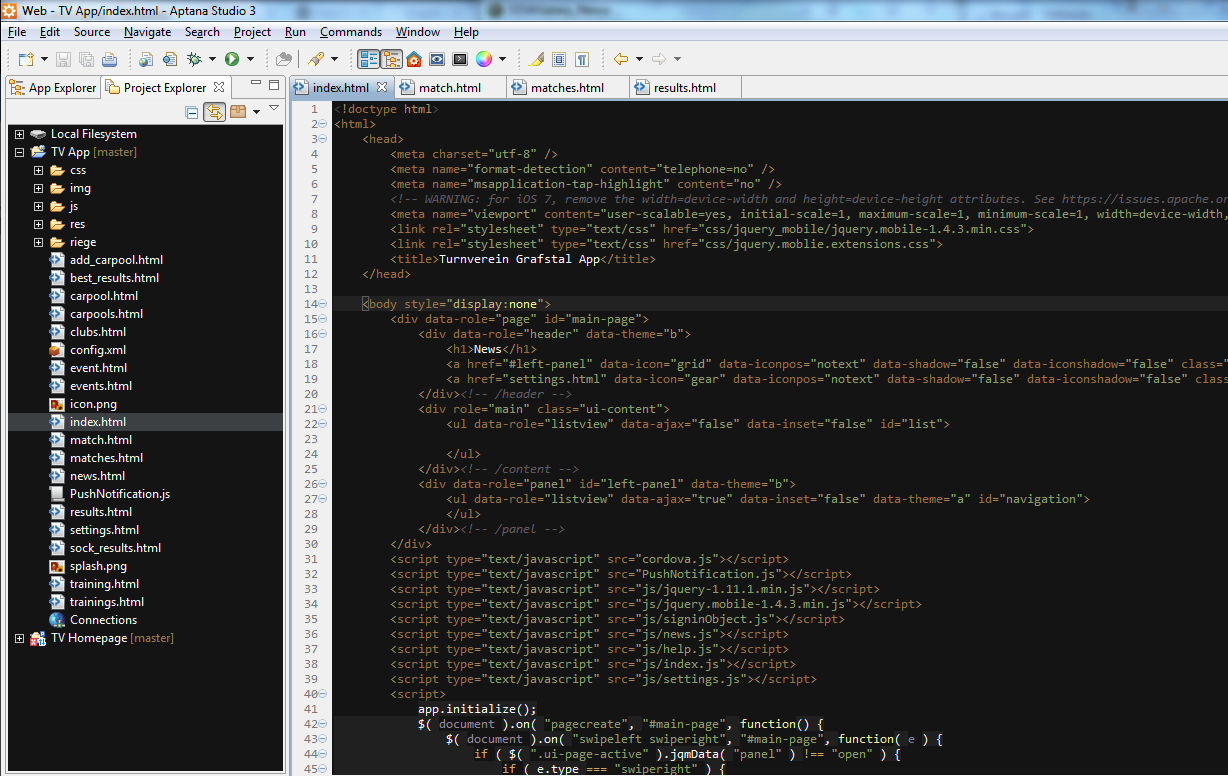
\includegraphics[scale=0.5]{images/aptana.png}
\caption{Aptana Studio}
\label{fig:aptana}
\end{figure}


\subsection{Versionierung}
Versionieriung ist in der Softwareentwicklung ein sehr wichtiges Thema, früher war das ein manueller Task, heute gibt es verschiedenste Tools, welche einem dabei unterstützen. In diesem Projekt wurde git (ref) verwendet, was eines der verbreitestens Versionierungstools ist. Das Remote Repository wurde auf Github (ref) erstellt. Es wurde geschaut, dass der Code jeden Abend auf das Repository geladen wurde, damit man auch gleich ein Backup hat.

\begin{figure}[h]
\centering
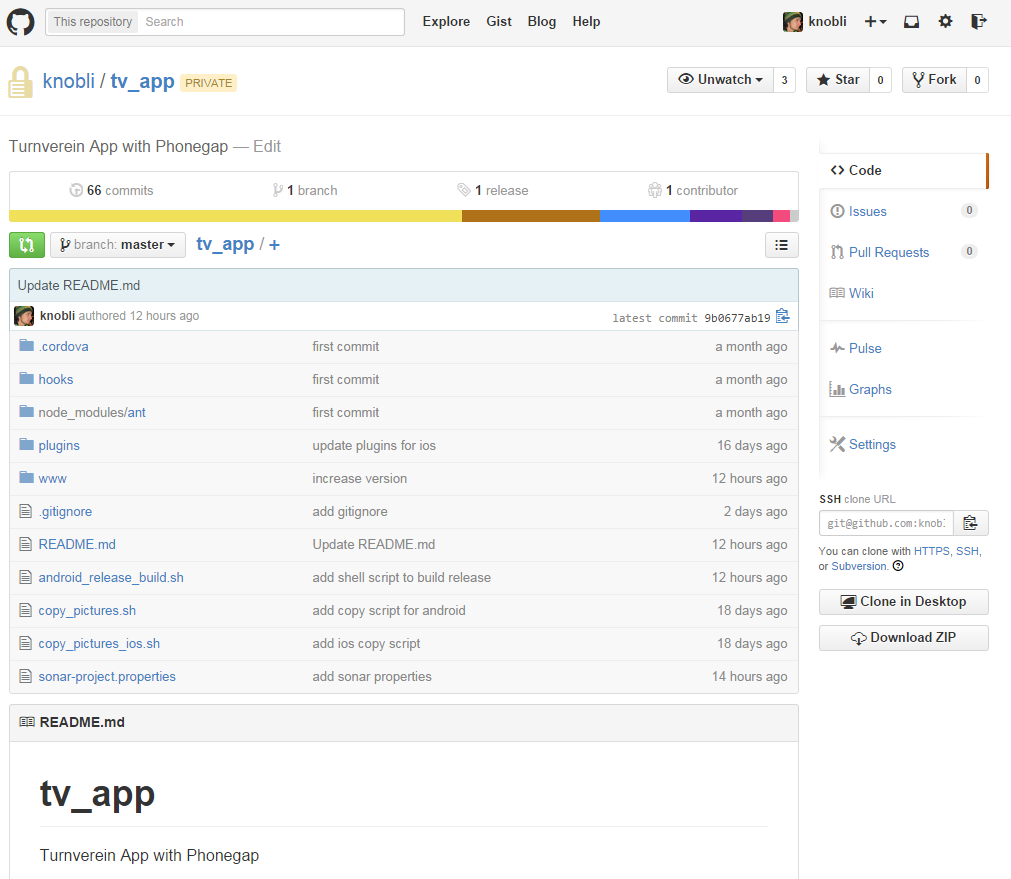
\includegraphics[scale=0.5]{images/github.png}
\caption{Github Repository}
\label{fig:github_repo}
\end{figure}

\newpage
\subsection{SDK - Software Development Kit}
Für die Entwicklung der App auf den beiden Plattformen Android und iOS wurden die dazugehörigen SDKs gebraucht, um die Applikation in einem Emulator laufen zu lassen. Vorallem bei Android, mit seinen diversenen Gerätevariationen, macht das Sinn, weil man beim Emulator jedes beliebige Device emulieren kann.

\begin{figure}[h]
\centering
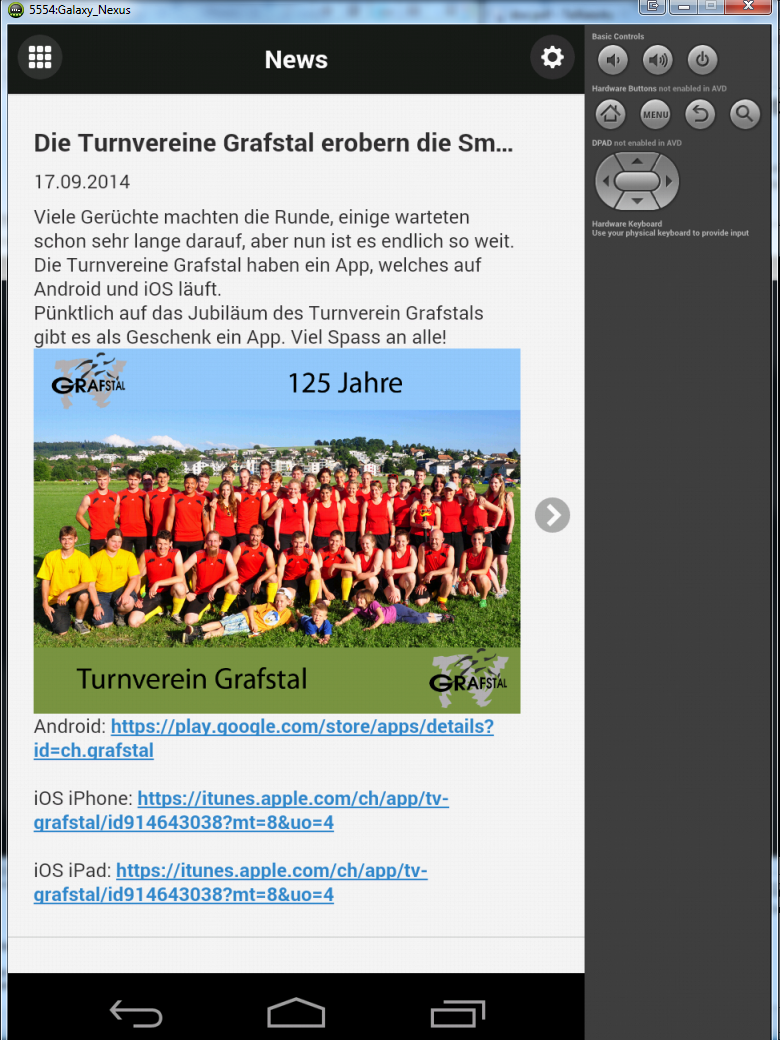
\includegraphics[scale=0.25]{images/android_emulator.png}
\caption{Android Emulator}
\label{fig:android_emulator}
\end{figure}

\FloatBarrier
\subsection{Webbrowser}
Die App wurde nicht nur auf Emulatoren getestet, sondern auch in Browsern. Dazu wurde auf Windows mit dem Google Chrome und auf Mac OSX mit Safari gearbeitet.

\subsection{Technische Geräte}
Push-Nachrichten können auf Emulatoren, wie auch in Webbrowsern nicht getestet werden, dazu benötigt man ein physisches Gerät. Die App wurde auf einem iPhone 4S, iPhone 5S, iPad und Samsung Ace getestet. Für die Entwicklung wurde ein Windows PC verwendet und damit XCode benutzt werden konnte, wurde zusätzlich noch auf einem iMac gearbeitet.

\newpage
\subsection{Testen - Analysieren}
Neben den Tests an Geräten, Emulatoren wurden auch noch automatisierte Tests und Analysen durchgeführt. Für die automatisierten Tests im Backend wurde PHPunit (siehe \cite{phpunit}) verwendet und für die statische Code Analyse wurde Sonar (siehe \cite{sonar}) mit dem PHP und Web Plugin (siehe Abbildung \ref{fig:sonar_backend} und \ref{fig:sonar_app}) aufgesetzt und verwendet. Damit das API direkt getestet werden konnte, wurde das Chrome App Advanced REST client (siehe Abbildung \ref{fig:advanced_rest_client}) verwendet.

\begin{figure}[h]
\centering
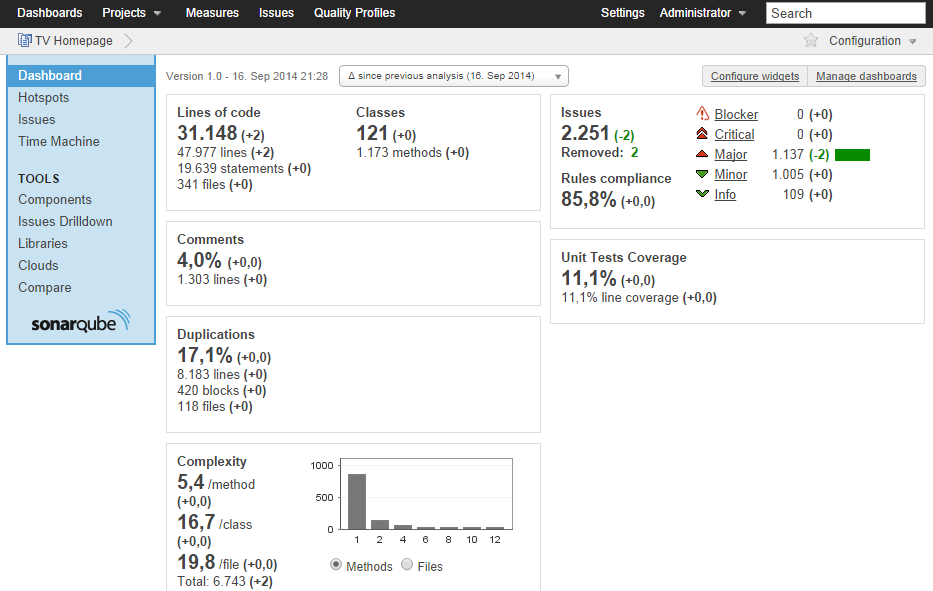
\includegraphics[scale=0.5]{images/sonar_backend.png}
\caption{Sonar - statische Code Analyse Backend}
\label{fig:sonar_backend}
\end{figure}

\begin{figure}[h]
\centering
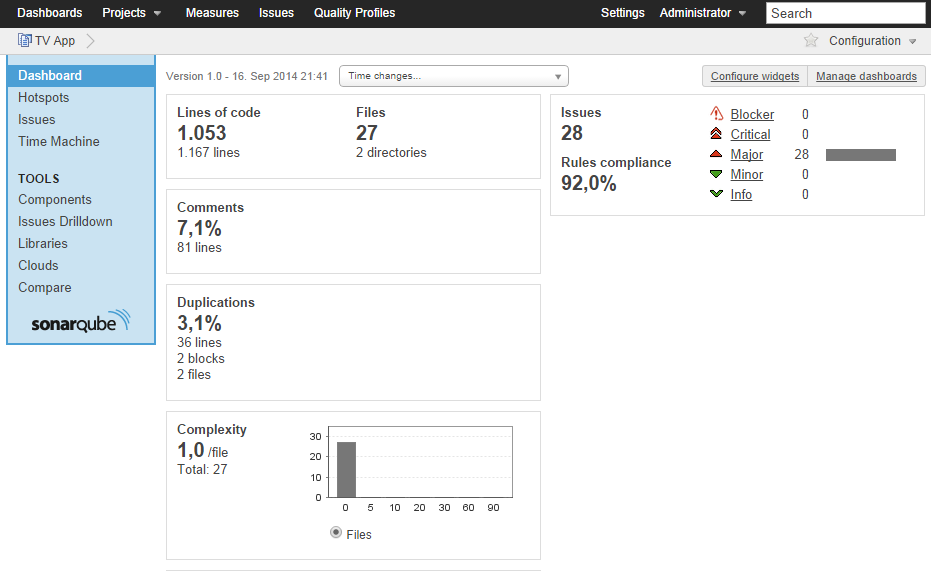
\includegraphics[scale=0.5]{images/sonar_app.png}
\caption{Sonar - statische Code Analyse App}
\label{fig:sonar_app}
\end{figure}

\begin{figure}[h]
\centering
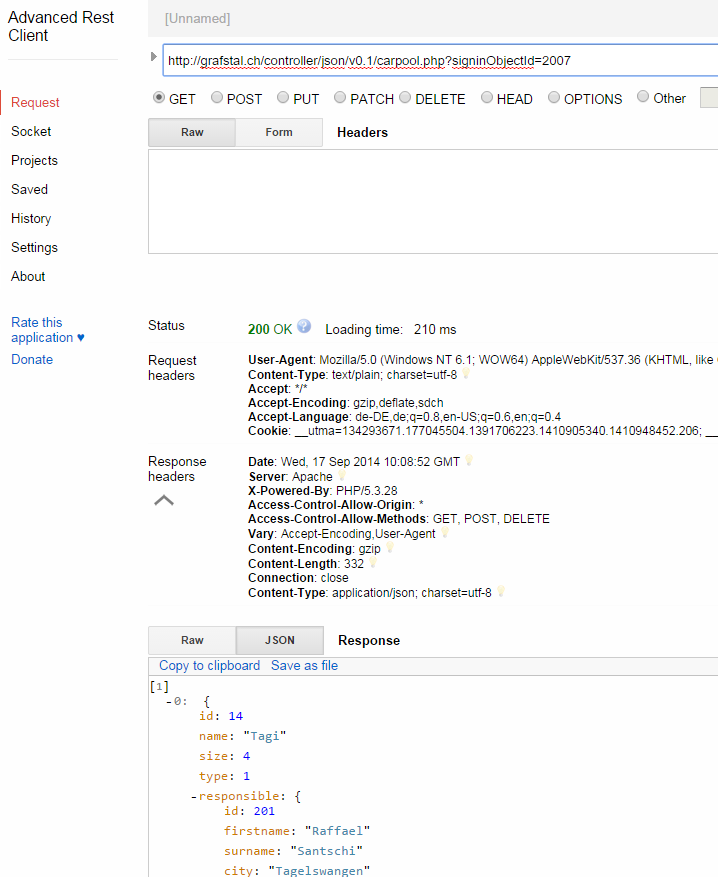
\includegraphics[scale=0.5]{images/advanced_rest_client.png}
\caption{Advanced Rest Client}
\label{fig:advanced_rest_client}
\end{figure}

\FloatBarrier


\clearpage
\section{Mobile App}\label{impl_moblie_app}
In diesem Unterkapitel werden neben einem detailierten Aufbau der App, die unterschiedlichen Provisioning Prozesse und das Refacotring des Backends beschrieben. Desweiteren wird eine Übersicht der Push-Nachricht Implementation vermittelt.

\subsection{Aufbau}
Das Menü (siehe Abbildung \ref{fig:navigation}) der App wurde sehr schlicht gehalten und sehr leicht erweiterbar gemacht. Da das Menü in verschiedenen Seiten gebraucht wird, werden die Elemente zentral verwaltet. Die Einträge News, Vereine und Veranstaltungen sind für alle Benutzer sichtbar, wenn auch mit anderem Inhalt und Design. Der Link zu den Resultaten ist nur für angemeldete Benutzer verfügbar.

\begin{figure}[h]
\centering
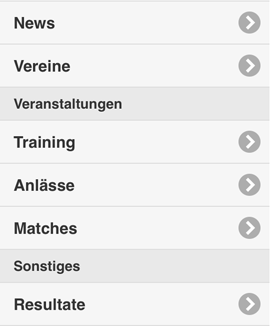
\includegraphics{images/app/navigation.png}
\caption{Navigation im App}
\label{fig:navigation}
\end{figure}

\FloatBarrier
\subsubsection{News}
Die News Seite (siehe Abbildung \ref{fig:app_news}) ist zu gleich auch die Startseite, wenn das App aufgemacht wird. Auf ihr werden die neuesten drei Berichte angezeigt. Das System ist wie auf der Homepage, die Elemente enthalten nur einen Einleitungstext und erst wenn man auf das Element klickt kann man den ganzen Bericht lesen. Dies hat den einfachen Grund, dass die Berichte zum Teil sehr lange sind und dann die anderen Berichte verloren gehen. Bei angemeldeten Mitgliedern wird zusätzlich noch die nächste Veranstaltung angezeigt, damit man sich sofort an- bzw. abmelden kann und wichtige Informationen nachschlagen kann.

\begin{figure}[h]
\centering

\includegraphics[scale=0.5]{images/app/news.png}
\caption{News Seite}
\label{fig:app_news}
\end{figure}

\FloatBarrier
\subsubsection{Vereine}
Die Vereine Seite (siehe Abbildung \ref{fig:app_vereine})  listet alle Vereine und Riegen der Turner Familie Grafstal auf. Wen man auf eine Riege klickt, erhält man zusätzliche Informationen, wie zum Beispiel die Trainingszeiten. Diese Seite enthält vorallem Informationen für die Öffentlichkeit oder ist ein Nachschlagewerk für Mitglieder.


\begin{figure}[h]
\centering
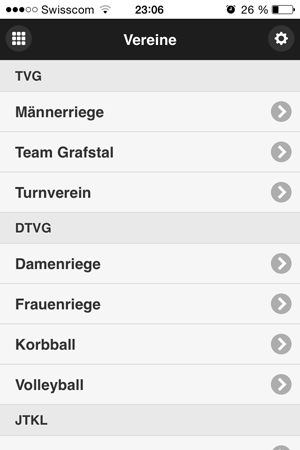
\includegraphics[scale=0.5]{images/app/vereine.png}
\caption{Vereinsseite}
\label{fig:app_vereine}
\end{figure}

\newpage
\FloatBarrier
\subsubsection{Veranstaltungen}
Die drei Veranstaltungsseiten sind alle gleich aufgebaut (siehe Abbildung \ref{fig:app_trainings}), sie zeigen die aktuellen Elemente mit Name, Datum, Zeit, Ort und Verantwortlichen. Falls der Benutzer angemeldet ist, wird durch Farbe angezeigt, ob er sich angemeldet (grün), abgemeldet (rot) oder nichts von beidem (grau) hat.
\begin{figure}[ht]
\centering
\subfigure[Anlässe (nicht angemeldet)]{
  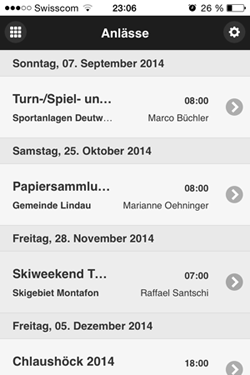
\includegraphics[scale=0.5]{images/app/events.png}
  \label{fig:app_events}
}
\subfigure[Trainings (angemeldet)]{
  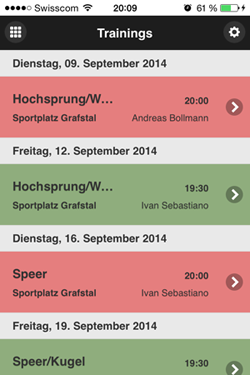
\includegraphics[scale=0.5]{images/app/trainings.png}
  \label{fig:app_trainings}
}
\label{fig:app_singinobjects}
\caption{Veranstaltungen}
\end{figure}

Wenn auf eine Veranstaltung geklickt wird, geht eine Detailansicht (siehe Abbildung \ref{fig:app_detail_event}) auf. In dieser Ansicht erhält man weitere Information, kann sich an- und abmelden und kommt auch zu den Fahrgemeinschaften. Die Information, wer sich angemeldet hat, sehen nur angemeldete Benutzer.

\begin{figure}[h]
\centering
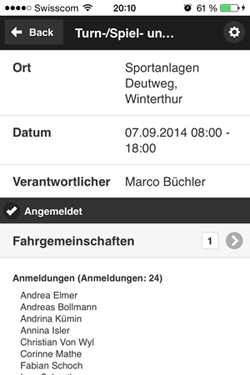
\includegraphics[scale=0.5]{images/app/event_detail.png}
\caption{Anlass Details}
\label{fig:app_detail_event}
\end{figure}

\newpage
\FloatBarrier
\subsubsection{Fahrgemeinschaften}
Bei jeder Veranstaltung können Fahrgemeinschaften erstellt werden, welche dann in der Übersicht (siehe Abbildung \ref{fig:app_carpools}) angezeigt werden. Man sieht den Namen, den Fahrer und den Wohnort vom Fahrer, zusätzlich sieht man noch, wie viele Plätze es noch frei hat oder dass man bereits angemeldet ist. In der Detailansicht (siehe Abbildung \ref{fig:app_carpool_detail}) kann man sich anmelden und erhält eine Liste der Mitfahrenden.
\begin{figure}[ht]
\centering
\subfigure[Fahrgemeinschaften]{
  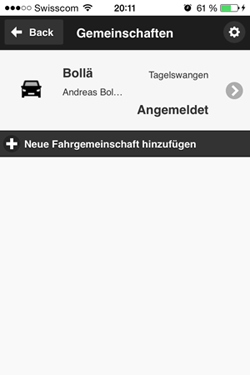
\includegraphics[scale=0.5]{images/app/carpools.png}
  \label{fig:app_carpools}
}
\subfigure[Fahrgemeinschaft Detail]{
  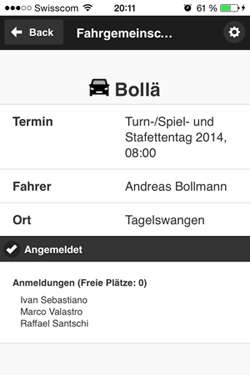
\includegraphics[scale=0.5]{images/app/carpool_detail.png}
  \label{fig:app_carpool_detail}
}
\label{fig:app_carpool_page}
\caption{Veranstaltungen}
\end{figure}

Im Formular (siehe Abbildung \ref{fig:app_add_carpool}) für die Erstellung einer neuen Fahrgemeinschaft muss man einen Namen angeben und kann den Typ der Gemeinschaft wählen, nur wenn es eine 'Car'-Fahrgemeinschaft ist, muss man die freien Plätze angeben.

\begin{figure}[h]
\centering
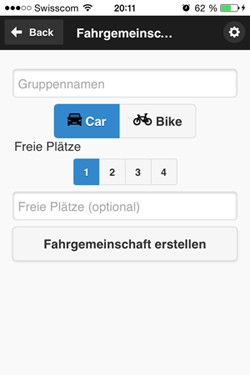
\includegraphics[scale=0.5]{images/app/add_carpool.png}
\caption{Fahrgemeinschaft erstellen}
\label{fig:app_add_carpool}
\end{figure}


\newpage
\FloatBarrier
\subsubsection{Resultate}
Unter Resultate (siehe Abbildung \ref{fig:app_results}) finden angemeldete Benutzer ihre Bestleistungen und die letzten Resultate.
\begin{figure}[h]
\centering
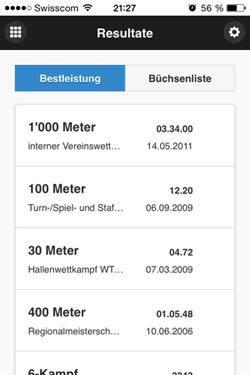
\includegraphics[scale=0.5]{images/app/results.png}
\caption{Resultate Seite}
\label{fig:app_results}
\end{figure}


\FloatBarrier
\subsubsection{Einstellungen}
In den Einstellungen kann sich der Benutzer nicht nur einloggen (siehe Abbildung \ref{fig:app_login}), sondern auch wählen, für welche Riege er die Matches, Anlässe und Trainings sehen möchte (siehe Abbildung \ref{fig:app_riege_setting}). Diese Filter werden dann auf die Veranstaltungsübersichtseiten angewendet.
\begin{figure}[ht]
\centering
\subfigure[Login Formular]{
  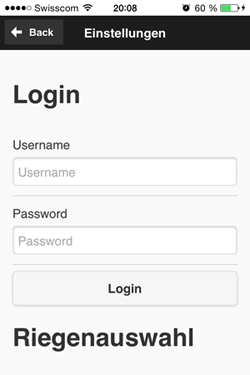
\includegraphics[scale=0.5]{images/app/settings1.png}
  \label{fig:app_login}
}
\subfigure[Riegen Einstellungen]{
  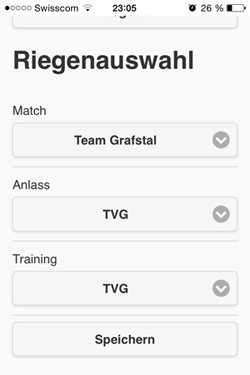
\includegraphics[scale=0.5]{images/app/settings2.png}
  \label{fig:app_riege_setting}
}
\label{fig:app_settings}
\caption{Einstellungen}
\end{figure}

\newpage
\FloatBarrier
\subsection{Javascript Funktionen}
Die Javascript Funktionen wurden möglichst generisch gewählt, damit man sie an verschiedenen Orten wiederverwenden kann. Mit diesem Anzatz ist man bei den verschiedenen Veranstaltungsseiten mehr wenig Code ausgekommen und es war einfach die nächste bevorstehende Veranstaltung auf der Startseite gleich anzuzeigen, wie in den anderen Seiten. Die Funktionen wurden in unterschiedliche Files geschrieben, welche nach ihrem Zweck benannt wurden.
\begin{itemize}
\item carpool.js: an- und abmelden bei Fahrgemeinschaften, anzeigen von Fahrgemeinschaften
\item help.js:  Datum formattieren,  Listen-Elemente erstellen, Navigationselemente
\item index.js: initialiseren der Push-Benachrichtigungen
\item news.js: Berichte laden
\item result.js: Resultate anzeigen
\item settings.js: Dropwdowns initialisieren, an- und abmelden, Riegenfilter setzen
\item signinObject.js: Veranstaltungen laden, Veranstaltungsdetails anzeigen, an- und abmelden bei Veranstaltungen 
\end{itemize}

\subsection{Login}
Da das Backend nur über eine HTTP-Verbindung verfügte und die Anmeldedaten nicht im localStorage  gespeichert werden sollten, wurde darauf verzichtet die Anmeldedaten bei jeder Anfrage an das Backend mitzusenden. Bei der Anmeldung wird die Mitglieder-ID gespeichert und dann bei einer Anfrage mitgeteilt. In einem späteren Projekt sollte diese Lösung durch ein Session-ID abgelöst werden.

\subsection{Provisioning Prozesse}
Die Entwicklung des Apps ist das eine, die Bereitstellung zum Download das andere. Phonegap hilft beim Provisioning vorallem bei Android, hier erstellt es, richtig konfiguriert, ein signiertes APK-Paket, welches in der Google Play Developer Console hochgeladen werden kann. Zuerst muss man sich jedoch einen Developer Account erstellen, danach kann man die Beschreibung und die Screenshots für das App hochladen. Das ganze dauert etwa 10 Minuten und 1 Stunden nach dem Absenden hat man sein App in Google Play. Es empfiehlt sich die App noch mit eine Absender-ID zu verknüpfen, damit man auch Statistiken über die Downloadzahlen sieht. (siehe dazu auch \cite{android_prov})\\
Bei Apple sieht das etwas anders aus, Phonegap kann kein Paket erstellen, es erstellt lediglich das Projekt. Diese Projekt muss man dann in XCode öffnen und von dort aus das Paket erstellen. Doch zuerst muss man einen Developer Account haben, diesen besitz man wahrscheindlich bereits, da man sonst nicht auf realen Geräten testen kann, zusätzlich muss man ein Distribution Zertifikate erstellen und in XCode hinzufügen. Danach muss man in iTunes Connect neben den gleiche Informationen wie bei Android, noch einige Angaben zu den Inhalten des Apps machen. Desweiteren muss man Review Informationen bereitstellen, dass heisst einen Test Benutzer und Informationen zum Entwicklung angeben. Erst wenn das App erfasst wurde, kann man in XCode ein Archiv erstellen und dieses direkt zu iTunes Connect hochladen. Nun werden schon die ersten Tests durchgeführt, ob zum Beispiel die Versionsnummern übereinstimmen und ob für jedes unterstütze Gerät Screenshots erfasst wurden. Falls dies nicht der Fall ist, wird das App abgelehnt und man muss die Dinge beheben. An diesem Punkt beginnt das warten, die durchschnittliche Review-Zeit beträgt 8 Tage. (siehe dazu auch \cite{apple_prov_apple} und \cite{apple_prov_ralf})

\FloatBarrier
\section{Backend}\label{impl_backend}

\subsection{Refactoring}
In diesem Unterkapitel wird kurz der vorgefundene Ist-Zustand beschrieben und danach die Schritte, welche unternommen wurden, um das Backend wartbarer und flexibler zu machen.

\subsubsection{Ist-Zustand}
Am Anfang dieses Projekts war in jeder Klasse HTML- mit PHP-Code verschmischt und SQL-Abfragen waren überall verstreut. Dies machte es schwierig den Code zu warten. Zusätzlich wurde jede save-, update-, load- und delete-Anweisung von Objekten, wenn es dann solche gab, selber implementiert, was sehr mühesam und unflexibel war. Zudem erweiterten ähnliche Objeke zwar eine Super-Klasse, teilten sich aber keine Tabelle und hatten somit auch verschiedene ID-Sequenzen.\\

Schnell wurde klar, dass man nicht mit diesem Stand ein API aufbauen sollte, welches dann von dem App angesprochen wird. Um den Code besser zu strukturieren, übersichtlicher und vorallem auch testbar zu machen, wurde ein Refacotring (siehe \cite{feathers2004working}) durchgeführt. Ausgehend von der Strategie für das Refactoring wurde Doctrine in das Projekt eingebunden. Doctrine ist, wie schon im Kapitel \ref{arch_backend} erklärt, ein ORM, welches richtig eingesetzt viel Arbeit abnehmen kann. Damit man Doctrine jedoch sinnvoll verwenden konnte, benötigte es zuerst einige Zeit für die Analyse und die Umstellungen.

\subsubsection{Refactoring}
Zuerst wurde geschaut, was zusammengefasst werden konnte. Alle Entities, bei welchen man sich anmelden kann, wurden ganz getreu dem 'Don’t repeat yourself' Prinzip als SigninObject zusammengefasst, da sie sehr viele gleiche Attribute und Funkionen haben. Im gleiche Zug wurde die Datenbank normalisiert, da zum Teil gleiche Ortnamen in verschiedenen Tabellen vorhanden waren. Da die einzelnen Typen jedoch auch spezifische Attribute haben, wurde eine Joined-Inheritance (siehe \cite{inheritance_java} und \cite{inheritance_doctrine}) angewendet, welche von vielen ORMs unterstützt wird. Die Joined-Inheritance basiert auf einer Grundtabelle, welche alle gemeinsamen Attribute beinhaltet und einer spezifischen Tabelle, welche die anderen Attribute beinhaltet. Die Tabellen werden über eine DiscriminatorColumn miteinander verknüpft. In diesem Konstrukt wurde auch ein Strategy-Pattern (siehe \cite{gof_book}) verwendet, um verschiedene Informationen im Kalender\footnote{Der Kalender (nicht in diesem Projekt entwickelt) kann über ein ics-File auf Geräten eingebunden werden.} anzuzeigen.\\

Dieser Umbau hat den grossen Vorteil, dass für jeden Veranstaltungstyp, sei dass ein Training, Match, Sitzung, Anlass oder Helfereinsatz, die gleiche Anmeldefunkion verwendet werden kann. Der Umbau machte sich auch bei der Entwicklung der Fahrgemeinschaftsverwaltung bezahlt, als diese nur ein mal implementiert werden musste.\\

\begin{figure}[h]
\centering
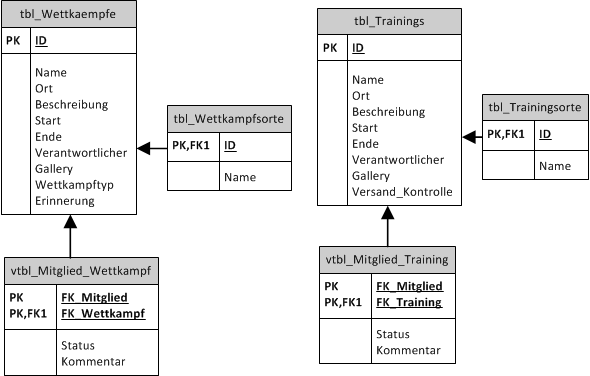
\includegraphics[scale=0.5]{images/visio/datenbankdiagramm_alt.png}
\caption{Datenbankdiagramm alt}
\label{fig:db_schema_alt}
\end{figure}

Das Datenbankdiagramm (siehe Abbildung \ref{fig:db_schema_alt}) zeigt einen kleinen Ausschnitt aus dem Datenbank Schema von früher. Jeder Veranstaltungstyp hatte seine eigene Ortstabelle und seine eigene Verknüpfungstabelle für die Anmeldungen. Wenn man sich nun vorstellt, dass dieses Konstrukt für die fünf verschiedenen Typen vorhanden war, kann man sich denken, wie viel Tabellen schon bereits nur für die Anmeldungen vorhanden waren. Nach dem Refactoring sah das Datenbankdiagramm (siehe Abbildung \ref{fig:db_schema_neu}) etwas einfacher aus, die Orte waren nun in einer Tabelle, die Anmeldungen auch und alle gemeinsamen Attribute wurden in der TerminObjekte-Tabelle gespeichert.

\begin{figure}[h]
\centering
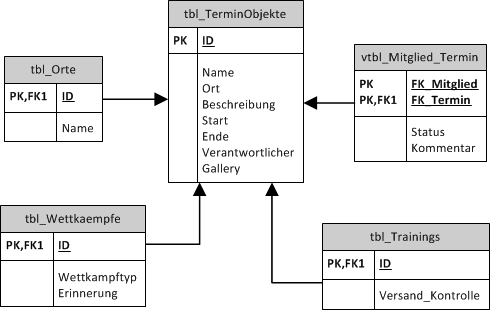
\includegraphics[scale=0.5]{images/visio/datenbankdiagramm_neu.png}
\caption{Datenbankdiagramm neu}
\label{fig:db_schema_neu}
\end{figure}

\FloatBarrier
Durch das Refactoring werden auch weniger SQL-Statments direkt in den Webseiten abgesetzt, es wird vermehrt\footnote{Nur an Orten, wo die Objekte innerhalb dieses Projektes angefasst wurden} mit Objekte gearbeitet. Ein Repository liefert die gewünschten Objekte zur Webseite, die Abfrage Logik ist somit zentralisiert. Das Repository arbeitet mit einer Object Query Language (OQL), bei welcher man nicht über die Spalten der Tabelle Werte abfragt, sondern über Attribute des Objekts. Eine Änderung des Spaltennamens hat somit keine grössere Auswirkung als eine kleine Änderung in der Entity.\\

Die Struktur sieht nach der Implementierung von Docrine, wie folgt aus:
\begin{itemize}
\item Entity: Attribute, Getter und Setter
\item Enity-Manager: persistiert, löscht und ladet Entities oder gibt das Repository der Entity zurück
\item Repository: spezifische Abfrage-Logik
\item Services\footnote{Services werden nicht von Doctrine zur Verfügung gestellt, wurden aber wegen ... implementiert (ref)}: Business-Logik
\end{itemize}

\newpage
\subsubsection{Facts and Figures}
Das Refactoring war zwar sehr Zeit aufwending, hat jedoch bei einigen Implementationen die Komplexität stark reduziert, Zeitersparnisse eingebracht und wird auch in Zukunft sehr viel erleichtern.
\begin{itemize}
\item Testabdeckung: Das Testen stellte sich voher als extrem schwierig heraus und ist nun mit den Kapselungen viel einfacher. Es konnte während des Projekts doch immerhin eine Testabdeckung von 11.1\% erreicht werden. Dieses Resultat wird natürlich noch sehr verfälsch durch Seiten und Funktionen, welche nicht Teil dieses Projekts waren.
\item Duplikate: Der Prozentsatz der duplizierten Linien konnte um fast 6\% reduziert werden, was etwa 4'000 Lines of code bedeutet.
\item Komplexität: Die Komplexität pro Klasse konnte von 40 auf 17 gesenkt werden.
\item Rule compliance: Die Rule compliance konnte um knapp 7\% gesteigert werden.
\item Issues: Über 3000 Issues, darunter alle kritischen und Blocker Issues, konnten behoben werden.
\end{itemize}


\subsection{Push-Nachrichten}
Das Versenden von Push-Nachrichten funktioniert bei iOS und Android ähnlich, jedoch sind die Vorbedingungen sehr unterschiedlich. Bei Android wird ein API-Key gebrauch, diesen kann man in der Google Developers Console erstellen kann. Dazu muss man ein Projekt erstellen und das 'Google Cloud Messaging for Android' aktivieren. Nun kann man einen neuen API-Key erstellen, welcher dann im Backend benötigt wird. Die Projektnummer ist zugleich die Sender ID und wird bei der Registierung des produktiven Apps über Phonegap benötigt. (siehe dazu \cite{android_push_android} und \cite{devgirl_push_android})\\


Bei iOS ist das etwas anders, als erstes braucht man ein Zertifikat, da nur ein Server mit diesem Zertifikat Push-Nachrichten an den APNS senden darf. Es gibt ein Zertifikat für den Entwicklungsserver und eines für den produktiven Server, über den Entwicklungsserver können nur verknüpfte\footnote{um das App auf einem Gerät zu testen, muss man es zuerst mit dem Developer Account verknüpfen} Geräte im Entwicklungsmodus erreicht werden. Zusätzlich muss für das Testen der Push-Nachrichten noch ein iOS App Development Provisioning Profile erstellt werden, welches dann auch mit dem Developer Account und den Test Geräten verknüpft wird. Bei der Erstellung der Zertifikate ist es wichtig, dass die App ID mit dem Projekt übereinstimmt, ansonsten kommen die Push-Nachrichten nicht an. Die Registierung des produktiven Apps über Phonegap ist ganz einfach und nicht Projekt spezifisch. (siehe dazu \cite{ios_push})\\

Nach der Registierung bei dem jeweiligen Servicen schickt das App den Geräteschlüssel mit der Mitglieder ID ans Backend, welches den Schlüssel mit der Verknüpfung zum Mitglied persistiert. Nun hat man den Schlüssel, welchen man für das gezielt Versenden von Push-Nachrichten benötigt.
\begin{figure}[ht]
\centering
\subfigure[Registration]{
  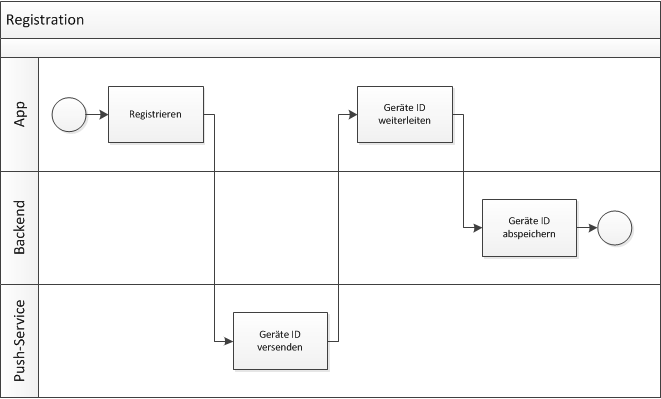
\includegraphics[scale=0.4]{images/visio/push_notification_flow_reg.png}
  \label{fig:push_notification_flow_reg}
}
\subfigure[Mitteilung versenden]{
  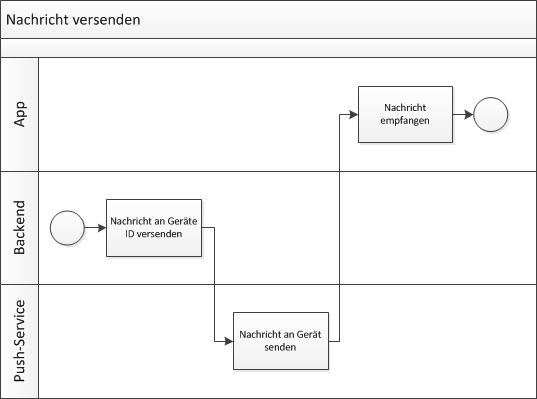
\includegraphics[scale=0.4]{images/visio/push_notification_flow_send.png}
  \label{fig:push_notification_flow_send}
}
\label{fig:app_settings}
\caption{Ablauf von Push-Nachrichten}
\end{figure}
